% Don't Do That: Keep your data in line with database constraints

% XXX XXX XXX This talk is boring. It's listing all the ways you can do stuff,
% without engaging examples of why you'd want to

\documentclass{beamer}
\usetheme{Madrid}
\usefonttheme{serif}
\usefonttheme{structuresmallcapsserif}
\usepackage{fancyvrb}
% \usepackage[font=small,labelfont=bf]{caption}

\begin{document}
\title{Don't Do That}
\subtitle{Ensuring data sanity with database constraints}
\author{Joshua Tolley}
\institute{End Point Corp.}

\frame{\titlepage}
%\frame{\tableofcontents}

%        \item Postgresql exclusion constraints
%        \item Why am I not talking about rules?
%        \item Refute Rails' "The app does it for me, so I don't have to worry about it in the database" agnosticism

\begin{frame}{ACID}
    \begin{figure}[t]
        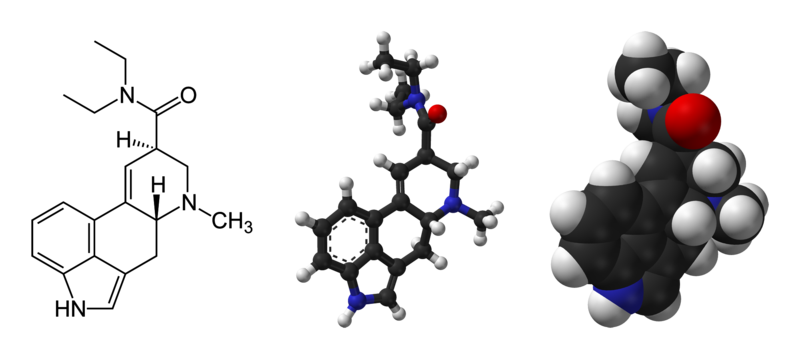
\includegraphics[width=0.8\textwidth]{lsd.png}
        \caption{Lysergic acid diethylamide, public domain image courtesy of Benjah-bmm27, Wikipedia}
    \end{figure}
\end{frame}

\begin{frame}{ACID}
    We've all heard about ACID:
    \begin{itemize}
        \item {\bf \color{red}Atomicity}: Operations are grouped into transactions; each transaction either succeeds or fails in its entirety
        \item {\bf \color{red}Consistency}: At the end of each transaction, the data meet all applicable constraints
        \item {\bf \color{red}Isolation}: Data from uncommitted transactions are invisible to all but the transaction that created them
        \item {\bf \color{red}Durability}: Kicking the power cord doesn't destroy your data
    \end{itemize}
    Most developers ignore atomicity and consistency, don't understand isolation, and take durability for granted.
\end{frame}

\begin{frame}{Just consistency, please}
    If you expect to hear about Atomicity, Isolation, or Durability, you're in the wrong room.
\end{frame}

\begin{frame}{Database constraints}
    You get consistency from database constraints. Constraints ensure your data remain sane, meaningful, and unambiguous. If you do them right.
\end{frame}

\begin{frame}
    \begin{block}{Why?}
        If you've ever dealt with ``bad'' data in the database, you'll understand why constraints are important
    \end{block}
\end{frame}

\begin{frame}{Database constraints}
    SQL databases maintain constraints in several ways:
    \begin{itemize}
        \item Check constraints
        \item Data type, including custom data types and domains
        \item UNIQUE, NOT NULL, DEFAULT (kinda)
        \item Primary and foreign keys
        \item Triggers
        \item Exclusion constraints
    \end{itemize}
\end{frame}

\begin{frame}[fragile]
    \frametitle{Check constraints}
    Check constraints simply verify a given expression
\small
    \begin{Verbatim}[fontfamily=courier]
 CREATE TABLE employee (
     manager_id INTEGER,  -- Employees with a manager
     team_id INTEGER,     -- must be assigned to a team
     salary FLOAT CHECK (salary > 0), -- Must be positive!
     CHECK ((manager_id IS NULL AND team_id IS NULL ) OR
        (manager_id IS NOT NULL AND team_id IS NOT NULL))
 );
       \end{Verbatim}
\end{frame}
\begin{frame}[fragile]
    \frametitle{Check constraints}
\small
    \begin{Verbatim}[fontfamily=courier]
  hal=# \d employee
            Table "public.employee"
     Column   |       Type       | Modifiers
  ------------+------------------+-----------
   manager_id | integer          |
   team_id    | integer          |
   salary     | double precision |
  Check constraints:
      "employee_check" CHECK (manager_id IS NULL AND
        team_id IS NULL OR manager_id IS NOT NULL AND
        team_id IS NOT NULL)
      "employee_salary_check" CHECK
        (salary > 0::double precision)
      \end{Verbatim}
\end{frame}

\begin{frame}[fragile]
    \frametitle{Check constraints}
    \small
    \begin{Verbatim}[fontfamily=courier]
   hal=# insert into employee (salary) values (-10);
   ERROR:  new row for relation "employee" violates check
     constraint "employee_salary_check"
   hal=# insert into employee (salary) values (10);
   INSERT 0 1
   hal=# select * from employee;
    manager_id | team_id | salary
   ------------+---------+--------
               |         |     10
   (1 row)
    \end{Verbatim}
\end{frame}

\begin{frame}[fragile]
    \frametitle{Check constraints}
    \small
    \begin{Verbatim}[fontfamily=courier]
   hal=# update employee set manager_id = 10;
   ERROR:  new row for relation "employee" violates check
     constraint "employee_check"
   hal=# update employee set team_id = 100;
   ERROR:  new row for relation "employee" violates check
     constraint "employee_check"
   hal=# update employee set team_id = 100,
     manager_id = 10;
   UPDATE 1
    \end{Verbatim}
\end{frame}

\begin{frame}{Data types}
    Many data types include parameters of one sort or another. Most have
    inherent limitations that act as constraints.
    \begin{itemize}
        \item Integers are limited to a specific range, and have no fractional part
        \item VARCHAR() fields are often limited in length
        \item ENUM types can contain only values from a defined set
        \item Date and time types can contain only {\bf{\color{red}VALID*}} dates
        \item Geometric, network, and other more complex types are also constrained
    \end{itemize}
    \vspace{10mm}
    {\footnotesize \color{red} \emph{* MySQL, are you listening?}}
\end{frame}

\begin{frame}[fragile]
    \frametitle{Custom data types}
    Many databases allow users to define their own data types
    \begin{block}{Composite data type}
    \vspace{2px}
    \begin{Verbatim}[fontfamily=courier]
   CREATE TYPE complex AS (
       r       double precision,
       i       double precision
   );
    \end{Verbatim}
    \vspace{2px}
    \end{block}
    \begin{block}{User-defined data type}
    \vspace{2px}
    \begin{Verbatim}[fontfamily=courier]
   CREATE TYPE box (
       INTERNALLENGTH = 16,
       INPUT = my_box_in_function,
       OUTPUT = my_box_out_function,
       ELEMENT = float4
   );
    \end{Verbatim}
    \vspace{2px}
    \end{block}
\end{frame}

\begin{frame}[fragile]
    \frametitle{Domains}
    The SQL standard includes \emph{domains}, which combine a given data type
    with one or more check constraints (more on check constraints later).
    \begin{Verbatim}[fontfamily=courier]
  CREATE DOMAIN us_postal_code AS TEXT
      CHECK(
          VALUE ~ '^\d{5}$'
          OR VALUE ~ '^\d{5}-\d{4}$'
  );
    \end{Verbatim}
\end{frame}

\begin{frame}{Column constraints}
    Column definitions can include constraints:
    \begin{itemize}
        \item UNIQUE
        \item NULL / NOT NULL
        \begin{itemize}
            \item DEFAULT (not really a constraint, but common with NOT NULL fields, and worth pointing out here)
        \end{itemize}
        \item PRIMARY KEY
        \item REFERENCES ... (foreign keys)
        \item CHECK
    \end{itemize}
\end{frame}

\begin{frame}{UNIQUE, [NOT] NULL}
    \begin{itemize}
        \item Unique columns must contain unqiue values
        \item ``Unique'' depends on the data type's definition of equality
        \item NULL means ``unknown'', so NULL != NULL, so UNIQUE columns can contain multiple NULLs
        \begin{itemize}
            \item ...so you might consider including a NOT NULL
            \item ...and perhaps a DEFAULT
        \end{itemize}
    \end{itemize}
    \begin{block}{Note}
        In PostgreSQL, UNIQUE is implemented with an index. Often, these are
        fields you'd likely want to index anyway. Users can declare the field ``UNIQUE'';
        the index will be created and named automatically.
    \end{block}
\end{frame}

\begin{frame}{PRIMARY KEY}
    Primary keys are UNIQUE and NOT NULL. Tables may have only one primary key, but many UNIQUE + NOT NULL columns.
\end{frame}

\begin{frame}[fragile]
    \frametitle{FOREIGN KEY}
    \begin{Verbatim}[fontfamily=courier]
CREATE TABLE employee (
  id SERIAL PRIMARY KEY,
  manager_id INTEGER REFERENCES employee (id),
  team_id INTEGER REFERENCES team (id),
  salary FLOAT CHECK (salary > 0),
  CHECK ((manager_id IS NULL AND team_id IS NULL ) OR
    (manager_id IS NOT NULL AND team_id IS NOT NULL))
 );
    \end{Verbatim}
    \begin{block}{Note} In PostgreSQL, columns referenced in a foreign key must be declared UNIQUE
    \end{block}
\end{frame}

\begin{frame}[fragile]
    \frametitle{FOREIGN KEY - Cascading}
    What happens when one of the teams or managers gets deleted?
    \begin{Verbatim}[fontfamily=courier]
  hal=# delete from team where id = 100;
  ERROR:  update or delete on table "team" violates
    foreign key constraint "team_fkey" on table
    "employee"
  DETAIL:  Key (id)=(100) is still referenced from
    table "employee".
    \end{Verbatim}
\end{frame}

\begin{frame}{FOREIGN KEY - Cascading}
    \texttt{ON UPDATE \emph{action}} and \texttt{ON DELETE \emph{action}}
    \begin{itemize}
        \item {\bf NO ACTION}: Throw an error saying that the action would break consistency
        \item {\bf RESTRICT}: Same as ``NO ACTION'', but not deferrable
        \item {\bf CASCADE}: Delete or update all rows referencing this row
        \item {\bf SET NULL}: Set referencing columns to NULL
        \item {\bf SET DEFAULT}: Set the referencing columns to their default values.
    \end{itemize}
\end{frame}

\begin{frame}[fragile]
    \frametitle{Cascading}
    \begin{Verbatim}[fontfamily=courier]
... team_id REFERENCES team (id) ON UPDATE CASCADE

 hal=# select * from employee;
  id | manager_id | team_id | salary
 ----+------------+---------+--------
   1 |          1 |     100 |     10
 (1 row)
 
 hal=# update team set id = 101 where id = 100;
 UPDATE 1
 hal=# select * from employee;
  id | manager_id | team_id | salary
 ----+------------+---------+--------
   1 |          1 |     101 |     10
 (1 row)
    \end{Verbatim}
\end{frame}

\begin{frame}[fragile]
    \frametitle{Deferred constraints}
    \begin{Verbatim}[fontfamily=courier]
 ... team_id REFERENCES team (id) DEFERRABLE
 hal=# begin;
 hal=# set constraints employee_team_id_fkey deferred;
 hal=# update team set id = 101;
 hal=# update employee set team_id = 101 where
    team_id = 100;
 hal=# commit;
 COMMIT
 hal=# select * from employee;
  id | manager_id | team_id | salary
 ----+------------+---------+--------
   1 |          1 |     101 |     10
 (1 row)
    \end{Verbatim}
\end{frame}

\begin{frame}{Multi-column constraints}
    These constraints can apply to multiple columns
    \begin{itemize}
        \item CREATE UNIQUE INDEX foo ON bar (baz, qux)
        \item CREATE TABLE CONSTRAINT foo\_fkey FOREIGN KEY (bar, baz) REFERENCES alpha (bar, baz)
    \end{itemize}
    \vspace{0.1\textheight}
    \begin{block}{Note}
        You can even set multi-column foreign keys so some of the columns can be NULL, but it's rarely used. Google ``foreign key match clause'' for more.
    \end{block}
\end{frame}

\begin{frame}{Advanced index-based constraints}
    Index-based constraints can become more flexible when used with functional or partial indexes
    \begin{itemize}
        \item CREATE UNIQUE INDEX ix1 ON foo (lower(bar));
        \item CREATE UNQIUE INDEX ix2 ON employee (name) WHERE (team\_id = 100);
    \end{itemize}
\end{frame}

\begin{frame}{Triggers}
    Triggers run user-defined functions (UDFs) when various things happen. Details of UDF programming are beyond this talk, but here's an example
\end{frame}

\begin{frame}[fragile]
    \footnotesize
    \begin{Verbatim}[fontfamily=courier]
CREATE FUNCTION sample() RETURNS TRIGGER AS $$
DECLARE
  msg TEXT; i INTEGER;
BEGIN
  IF NEW.jurisdiction_id IS NOT NULL AND NOT EXISTS (
    SELECT 1 FROM places p
      JOIN places_types pt ON (pt.place_id = p.id)
      JOIN codes c ON (c.the_code = 'J' AND c.id = pt.type_id)
    WHERE p.id = NEW.jurisdiction_id
  ) THEN
    RAISE EXCEPTION 'Error. Place % is not a jurisdiction.',
        NEW.jurisdiction_id;
    RETURN NULL;
  END IF;
  RETURN NEW;
END;
$$ LANGUAGE plpgsql;

CREATE TRIGGER sample_trigger BEFORE INSERT OR UPDATE
    ON some_table FOR EACH ROW EXECUTE PROCEDURE sample();
    \end{Verbatim}
\end{frame}

\begin{frame}{Triggers}
    \begin{block}{Note}
        PostgreSQL has at least 18 different languages available for
        user-defined functions. These include PL/pgSQL (like Oracle's PL/SQL),
        Perl, Python, Tcl, Javascript, Lua, Java, Ruby, and LOLCODE. Not all
        these languages support triggers.
    \end{block}
    \vspace{0.1\textheight}

    Note that defining a trigger to validate data will \emph{not} automatically validate the data already in the table.
\end{frame}

\begin{frame}{Triggers}
    Triggers can do all kinds of neat things:
    \begin{itemize}
        \item Validate new and modified data
        \item Log users' behavior
        \item Calculate hidden fields
        \item Make views that work like tables
        \item Launch the missiles
    \end{itemize}
\end{frame}

\begin{frame}{Why PostgreSQL Rocks: Exclusion Constraints}
    A UNIQUE constraint can be generalized. Unique constraints say ``don't allow
    data where the equality operator for this data type returns true for a new
    row and some existing row''. What if we weren't limited to the equality
    operator?
\end{frame}

\begin{frame}[fragile]
    \frametitle{Why PostgreSQL Rocks: Exclusion Constraints}
    \begin{Verbatim}[fontfamily=courier]
  hal=# CREATE TABLE circles (
      my_circle circle,
      name text,
      EXCLUDE USING gist ( my_circle WITH && )
  );
    \end{Verbatim}
    \vspace{2px}
    \&\& is the ``overlaps'' operator for PostgreSQL's native circle type. So this says ``don't allow circles to overlap.''

    \begin{block}{Note}
        Only PostgreSQL allows you to do this.
    \end{block}
\end{frame}

\begin{frame}[fragile]
    \frametitle{Exclusion Constraints}
    \begin{Verbatim}[fontfamily=courier]
  hal=# insert into circles values
    ('0, 0, 10', 'first);
  INSERT 0 1
  hal=# select * from circles ;
  my_circle  | name
  ------------+-------
  <(0,0),10> | first
  (1 row)
  
  hal=# insert into circles values
    ('5,0,10', 'second');
  ERROR:  conflicting key value violates exclusion
    constraint "circles_my_circle_excl"
  DETAIL:  Key (my_circle)=(<(5,0),10>) conflicts
    with existing key (my_circle)=(<(0,0),10>).
    \end{Verbatim}
\end{frame}

\begin{frame}{Exclusion Constraints}
    Other possible uses:
    \begin{itemize}
        \item Don't put the lions and the zebras in the same zoo enclosure
        \item Prevent overlapping time ranges in a scheduling application
        \item Weird data types offer all kinds of possibilities
    \end{itemize}
\end{frame}

\begin{frame}{Refutation and Rebuttal}
    Some application frameworks{\color{red}*} claim they handle all data validation in the application, so the database doesn't need to worry about it. What could possibly go wrong?
    \\
    \vspace{0.5\textheight}
    {\footnotesize \color{red} \emph{* Rails, I'm talking to you}}
\end{frame}

\begin{frame}{Refutation and Rebuttal}
    What if\ldots
    \begin{itemize}
        \item some other process access the database outside your application?
        \item the database were smart enough to optimize queries based on the constraints you declared, but you didn't declare them?
        \item the database could process the constraints faster than the application can?
        \item the constraints could be cleaner, simpler, and more straightforward in SQL?
    \end{itemize}
\end{frame}

\begin{frame}{Please...}
    \centering
    { 
        
\includegraphics[width=0.8\textwidth]{snake.jpg}
        \\
        Don't let your data run wild. Who knows what it might do...
    }
\end{frame}

\end{document}
